\documentclass[pstricks]{amsart}
\usepackage{amsmath}
\usepackage{amssymb}
\usepackage{multirow}
\usepackage{hyperref}
\usepackage{tikz,pgf}
\usepackage[margin=.5in]{geometry}
\usepackage{floatrow}
\usepackage{caption}
\floatsetup[table]{capposition=top}

\usetikzlibrary{calc}

\usetikzlibrary{intersections, calc, fpu, decorations.pathreplacing}

\def\major{2,2,1,2,2,2,1}
\def\harmonic{2, 1, 2, 2, 1, 3, 1}
\def\melodic{2, 1, 2, 2, 2, 2, 1}

\author{cuppajoeman}
\thanks{test}

\begin{document}

Conversion from standard notation to semitones - Made by cuppajoeman - \url{http://cuppajoeman.com}

\vspace{.15cm}


\begin{center}
\scalebox{2}{
$\begin{array}{ccccccccccccc}
    C& \cdot& D& \cdot& E& F& \cdot& G& \cdot& A& \cdot& B & C \\
    \updownarrow & \updownarrow & \updownarrow & \updownarrow & \updownarrow & \updownarrow & \updownarrow & \updownarrow & \updownarrow & \updownarrow & \updownarrow & \updownarrow & \updownarrow \\
    0^{\star} & 1^{\star} & 2^{\star} & 3^{\star} & 4^{\star} & 5^{\star} & 6^{\star} & 7^{\star} & 8^{\star} & 9^{\star} & 10^{\star} & 11^{\star} & 0^{\star}\\
\end{array} $
}
\end{center}

\vspace{.30cm}
\begin{center}
  \line(1,0){300}
\end{center}
\vspace{.30cm}

\begin{center}
  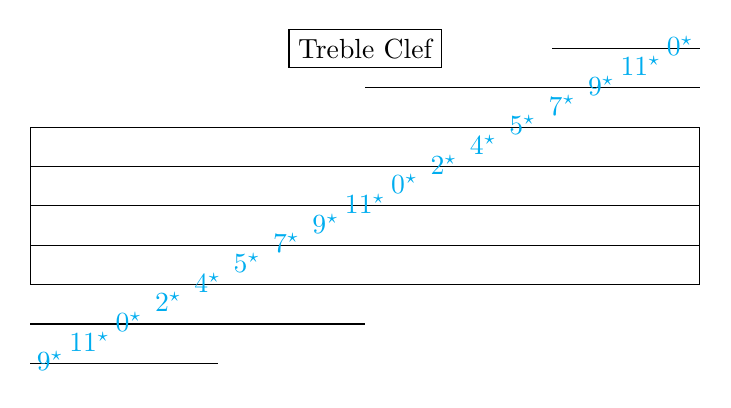
\begin{tikzpicture}[scale=0.5]
  % Label diagram
  \node[draw] at (8.5,6) {Treble Clef};
  % Ledger lines
  \draw (13.25,6) -- (17,6);
  % Main section
  \draw (8.5,5) -- (17,5);
  \foreach \y in {0, 1, 2, 3, 4} {
    \draw (0, \y) -- (17, \y);
  }
  \draw (0,0) -- (0, 4);
  \draw (17,0) -- (17, 4);
  %\draw [step=1.0,black] (0,0) grid (17,4);
  % Lower lines
  \draw (0,-1) -- (8.5,-1);
  \draw (0,-2) -- (4.75,-2);
  % Counter
  \edef\counter{0}
  \foreach \x in {9, 11, 0, 2, 4, 5, 7, 9, 11, 0, 2, 4, 5, 7 , 9, 11, 0} {
    %\node[draw,circle,fill=white,minimum size=2] at (\counter + .5, \counter * .5 - 2) {\huge\x};
    \node[text=cyan] at (\counter + .5, \counter * .5 - 1.95) {$\x^{\star}$};
    \pgfmathparse{\counter+1}
    \xdef\counter{\pgfmathresult}
  }
    %\draw at (\x + .5, \x * .5) {\x}
\end{tikzpicture}
\hfill
  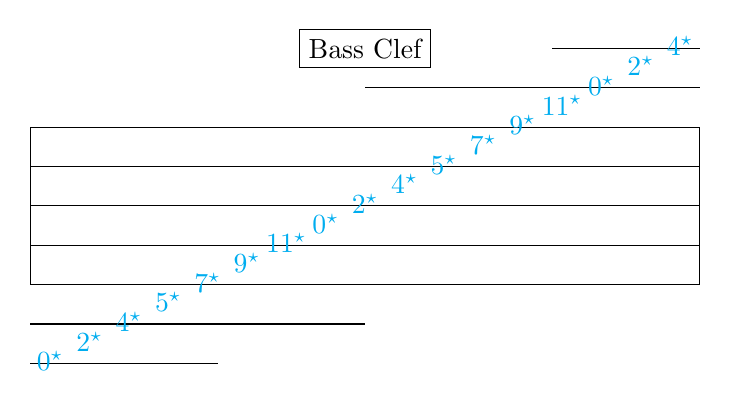
\begin{tikzpicture}[scale=0.5]
  % Label diagram
  \node[draw] at (8.5,6) {Bass Clef};
  % Ledger lines
  \draw (13.25,6) -- (17,6);
  % Main section
  \draw (8.5,5) -- (17,5);
  \foreach \y in {0, 1, 2, 3, 4} {
    \draw (0, \y) -- (17, \y);
  }
  \draw (0,0) -- (0, 4);
  \draw (17,0) -- (17, 4);
  %\draw [step=1.0,black] (0,0) grid (17,4);
  % Lower lines
  \draw (0,-1) -- (8.5,-1);
  \draw (0,-2) -- (4.75,-2);
  % Counter
  \edef\counter{0}
  \foreach \x in {0, 2, 4, 5, 7, 9, 11, 0, 2, 4, 5, 7 , 9, 11, 0, 2, 4} {
    %\node[draw,circle,fill=white,minimum size=2] at (\counter + .5, \counter * .5 - 2) {\huge\x};
    \node[text=cyan] at (\counter + .5, \counter * .5 - 1.95) {$\x^{\star}$};
    \pgfmathparse{\counter+1}
    \xdef\counter{\pgfmathresult}
  }
    %\draw at (\x + .5, \x * .5) {\x}
  \end{tikzpicture}
\end{center}

\vspace{.30cm}
\begin{center}
  \line(1,0){300}
\end{center}
\vspace{.30cm}

\begin{center}
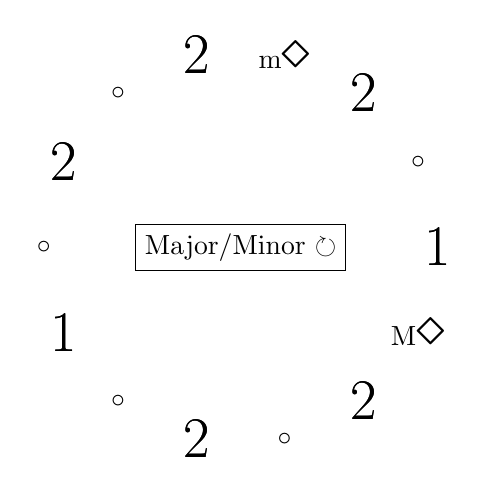
\begin{tikzpicture}
  \foreach \a [count=\c,evaluate=\c as \y using {{\major}[\c-1]}] in  {1,2,...,7}{
    \draw (\a*360/7*-1: 2.5) node {\huge{\y}};
    \draw (\a*360/7*-1: 2.5) node {\huge{\y}};
  }
  \foreach \a in  {1,2,3,4,6}{
    \draw (\a*360/7*-1 + 1/2*360/7*-1: 2.5) node {$\circ$};
  }
  \draw (0.5*360/7*-1: 2.5) node {M\huge{$\diamond$}};
  \draw (5.5*360/7*-1: 2.5) node {m\huge{$\diamond$}};
  \node[draw] at (0,0) {Major/Minor $\circlearrowright$};
\end{tikzpicture}
\hfill
\begin{tikzpicture}
  \foreach \a [count=\c,evaluate=\c as \y using {{\harmonic}[\c-1]}] in  {1,2,...,7}{
    \draw (\a*360/7*-1: 2.5) node {\huge{\y}};
  }
  \foreach \a in  {1,2,3,4,5,6}{
    \draw (\a*360/7*-1 + 1/2*360/7*-1: 2.5) node {$\circ$};
  }
  \draw (0.5*360/7*-1: 2.5) node {\huge{$\diamond$}};
  \node[draw] at (0,0) {Harmonic $\circlearrowright$};
\end{tikzpicture}\hfill
\begin{tikzpicture}
  \foreach \a [count=\c,evaluate=\c as \y using {{\melodic}[\c-1]}] in  {1,2,...,7}{
    \draw (\a*360/7*-1: 2.5) node {\huge{\y}};
  }
  \foreach \a in  {1,2,3,4,5,6}{
    \draw (\a*360/7*-1 + 1/2*360/7*-1: 2.5) node {$\circ$};
  }
  \draw (0.5*360/7*-1: 2.5) node {\huge{$\diamond$}};
  \node[draw] at (0,0) {Melodic $\circlearrowright$};
\end{tikzpicture}
\end{center}

\vspace{.30cm}
\begin{center}
  \line(1,0){300}
\end{center}
\vspace{.30cm}

% Please add the following required packages to your document preamble:
% \usepackage{multirow}
\begin{table}[h]
  \centering
  \begin{tabular}{|c|c|c|c|}
    \hline
    \begin{tabular}[c]{@{}c@{}}Number of\\ semitones\end{tabular} & Name (Minor, Major or Perfect) & Short             & Name (Diminished or Augmented) \\ \hline
    0                                                             & Perfect unison                 & P1                & Diminished second              \\ \hline
    1                                                             & Minor second                   & m2                & Augmented unison               \\ \hline
    2                                                             & Major second                   & M2                & Diminished third               \\ \hline
    3                                                             & Minor third                    & m3                & Augmented second               \\ \hline
    4                                                             & Major third                    & M3                & Diminished fourth              \\ \hline
    5                                                             & Perfect fourth                 & P4                & Augmented third                \\ \hline
    \multirow{2}{*}{6}                                            & \multirow{2}{*}{}              & \multirow{2}{*}{} & Tritone|Diminished fifth       \\ \cline{4-4} 
                                                                  &                                &                   & Tritone|Augmented fourth       \\ \hline
    7                                                             & Perfect fifth                  & P5                & Diminished sixth               \\ \hline
    8                                                             & Minor sixth                    & m6                & Augmented fifth                \\ \hline
    9                                                             & Major sixth                    & M6                & Diminished seventh             \\ \hline
    10                                                            & Minor seventh                  & m7                & Augmented sixth                \\ \hline
    11                                                            & Major seventh                  & M7                & Diminished octave              \\ \hline
    12                                                            & Octave|Perfect octave          & P8                & Augmented seventh              \\ \hline
  \end{tabular}
\end{table}


\begin{table}[]
\renewcommand{\arraystretch}{2}
\begin{tabular}{|c|c|}
\hline
 $\{0,7\}$ & $X$ Power Chord , $X_5$ \\ \hline
 $\{0,4,7\}$ & $X$ major triad , $X_M$ \\ \hline
 $\{0,3,7\}$ & $X$ minor triad , $X_m$ \\ \hline
 $\{0,3,6\}$ & $X$ diminished triad , $X^\circ$ \\ \hline
  $\{0,2,7\}$& $X$ suspended second, $X_{S2}$\\ \hline
  $\{0,5,7\}$& $X$ suspended fourth, $X_{S4}$\\ \hline
 $X_Z \cup \{9\}$ & $X^6_Z, \quad Z \in \{ M, m, \epsilon \}$  \\ \hline
 $X^\circ \cup \{9\}$ &  $X$ diminished, X$^{\circ 7}$ ,$X^{7}_{\text{dim}}$ \\ \hline
 $X_Z \cup \{10\}$ & $X^7_Z, \quad Z \in \{  m, S2, S4 \}$  \\ \hline
 $X_M \cup \{10\}$ & $X^7$ \\ \hline
 $X^\circ \cup \{10\}$ & $X$ half diminished      , $X^{\varnothing 7}$        , $X^{7\flat 5}_{\text{min}} $  \\ \hline
 $X_M \cup \{11\}$ & $X$ major 7              , $X_M^7$ , $X\Delta$ or $X^7\Delta$ \\ \hline
 $X_m \cup \{11\}$ & $X$ minor major 7        , $X_{\text{min \& maj}}^7$,     $X – \Delta7$    \\ \hline
 $X_Z^7 \cup \{2\}$ & $X^9_{\text{Z}}$ \\ \hline
 $X^7 \cup \{1\}$ & $X^{7\flat 9}$ \\ \hline
  $X^9_Z \cup \{5\}$&  $X^{11}_Z, \quad Z \in \{ M, m, \epsilon \}$ \\ \hline
\end{tabular}
\caption*{Common Chords}
\end{table}
\renewcommand{\arraystretch}{1}






\end{document}
